\documentclass{article}

% if you need to pass options to natbib, use, e.g.:
%     \PassOptionsToPackage{numbers, compress}{natbib}
% before loading neurips_2020

% ready for submission
% \usepackage{neurips_2020}

% to compile a preprint version, e.g., for submission to arXiv, add add the
% [preprint] option:
    % \usepackage[preprint, nonatbib]{neurips_2020}

% to compile a camera-ready version, add the [final] option, e.g.:
\usepackage[final, nonatbib]{neurips_2020}

% to avoid loading the natbib package, add option nonatbib:
% \usepackage[nonatbib]{neurips_2020}

\usepackage[utf8]{inputenc} % allow utf-8 input
\usepackage[T1]{fontenc}    % use 8-bit T1 fonts
\usepackage{hyperref}       % hyperlinks
\usepackage{url}            % simple URL typesetting
\usepackage{booktabs}       % professional-quality tables
\usepackage{amsfonts}       % blackboard math symbols
\usepackage{nicefrac}       % compact symbols for 1/2, etc.
\usepackage{microtype}      % microtypography
\usepackage{graphicx}
\graphicspath{{"../results/"}}

\title{Predicting forest carbon stocks in the contiguous U.S.}

% The \author macro works with any number of authors. There are two commands
% used to separate the names and addresses of multiple authors: \And and \AND.
%
% Using \And between authors leaves it to LaTeX to determine where to break the
% lines. Using \AND forces a line break at that point. So, if LaTeX puts 3 of 4
% authors names on the first line, and the last on the second line, try using
% \AND instead of \And before the third author name.

\author{%
  Erich Trieschman\\
  Department of Statistics, M.S.\\
  Stanford University\\
  Stanford, CA 94305\\
  \texttt{etriesch@stanford.edu} \\
}

\begin{document}

\maketitle

\begin{abstract}
In this project I explore the viability of statistical models to predict forest biomass. These models are trained on an existing dataset of forest biomass measurements collected by the USDA Forest Service and utilize features generated from remote sensing data collected by the NASA MODIS sensor. I find that several aggregate remote sensing features are predictive of county-panel-level forest biomass estimates, achieving an $R^2$ of 0.60. Specifically, more variable land surface temperature and NDVI are associated with lower forest biomass, and a higher minimum land surface temperature is associated with lower forest biomass. My aim with these statitical models is to support predictions under three scenarios: in regions with existing measurements, in regions without existing measurements, and forward in time. I find that the Random Forest Regressor yields the lowest RMSE in cross validation across all three of these scenarios. For the first scenario only, I find that the test data and test predictions are not statistically distinct, which offers further support for this model's use in making broad scale forest biomass predictions.
\end{abstract}

%------------------------------------------------------------------------
\section{Introduction}
\label{sec:intro}
Protecting and properly managing our natural resources is an important step in addressing the risks of climate change. Forests are one such resource with a portfolio of environmental and economic benefits, from temperature and moisture attenuation, to timber and horticulture. This resource has been directly impacted by humans, through urbanization and agricultural expansion, and indirectly through droughts, fires, and other risks posed by climate change. Monitoring our forests and properly accounting for their extent and health could help improve their management and strengthen their protection.

This calls for the need of precise, low-cost approaches for estimating the amount of carbon stored in a forest. In this project I explore the viability of statistical models to quantify forest biomass. These models leverage a current dataset of forest biomass measurement, collected through intensive sampling campaigns run by the USDA Forest Service, to produce higher frequency estimates with the help of low-cost remote sensing data collected by the NASA modis sensor. 

I first use regression analysis to interpret the remote sensing features I develop for my model. I then use  cross validation to select the highest-performing statistical model for several distinct use cases, including out-of-region prediction and future prediction. The end result of this research is a series of trained models, evaluated on held-out data, for use in predicting forest biomass in these settings.

%------------------------------------------------------------------------
\subsection{Related work}

There there is much established literature on forest biomass prediction. For example, Han et al. and Li et al. both evaluate several machine learning algorithms to estimate forest biomass, using Sentilel-1 and Landsat 8 satellites \cite{Han_2022, Li_2020}. Han et al. achieve best performance with Random Forest Regressors, while Li et al. achieve best performance with XGBoost. Bjork et al. adopts deeper learning techniques for a similar aim: to estimate forest biomass from airborne laser scanning (ALS) \cite{Bjork_2021}. Bjork et al. adopt a sequential modeling approach first relating ground measurements to ALS and then the resulting mapping to Sentinel-1 satellite imagery. The team's model leverages generative adversarial networks and convolutional filters to utilize the spatial structure of these maps in their model training. 

Saarela et al. and Naik et al. evaluate newer remote sensing layers for incremental benefits to forest biomass estimates \cite{Saarela_2020, Naik_2021}. Saarela uses LiDAR and field data to estimate aboveground biomass and associated uncertainty, while Naik uses multispectral remote sensing data; both papers find improvements in model accuracy with this additional data.

And Vorster et al. contributes to this body of research by exploring how allometric equations can improve estimates of uncertainty in biomass estimates made from remote sensing \cite{Vorster_2020}. Vorster et al. develop biomass estimates using allometric equations at tree, plot, and landscape level and relate each to satellite imagery. The team then combines uncertainty estimates from both their prediction model and the allometric equations themselves. 

%------------------------------------------------------------------------
\section{Dataset}
\label{sec:data}

In this research, I compile a dataset of county-level biomass estimates from the USDA Forest Service and spatio-temporal aggregated satellite imagery data from NASA's Moderate Resolution Imaging Spectoradiometer (MODIS). I describe both data sources and their processing in more detail below. 

Since the late 1930s, the USDA Forest Service has surveyed US forests at the county level through the Forest Inventory and Analysis program (USDA FS FIA). The FIA surveys a forest over 5-7 year periods through a random sampling procedure, and provides panel-county-level forest biomass estimates to the public through an online portal called The Design and Analysis Toolkit for Inventory and Monitoring (DATIM) \cite{DATIM}. In this analysis I use the FIA's estimate of aboveground forest biomass measured in short tons of carbon. I provide a map of county-level forest biomass for the latest panel of data in each county in Figure \ref{fig:biomass}.

\begin{figure}[!htbp]
  \centering
  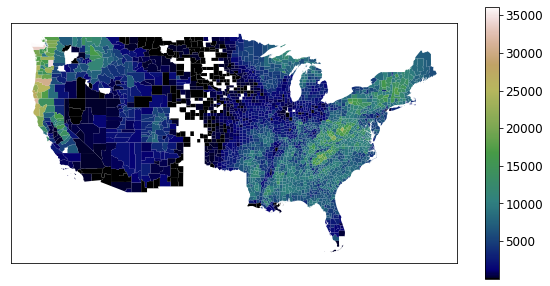
\includegraphics[width=.8\linewidth]{"./fig_biomass.png"}
  \caption{\label{fig:biomass} USDA FS aboveground forest biomass (Short tons / km2), in most recent USDA FS panel}
\end{figure}

The NASA MODIS satellite-based sensor is on board two satellites tracking land and ocean surface climate measurements, launched in the late 1990s and early 2000s respectively. For broader scale use, NASA provides Level 3 gridded data products built from lower-level products relying on the raw sensor readings. In this analysis, I use monthly binned L3 readings at a 5600m grid scale, accessed through NASA's EarthDataSearch platform \cite{modis_ndvi} \cite{modis_lst}. In this analysis I consider mean monthly land surface daytime temperature (LST) and mean monthly normalized difference vegetation index (NDVI). NDVI is roughly a measure of how green the land looks from space.

I create a uniform analysis dataset for this research by aggregating NASA MODIS data across space and time. I begin by aggregating MODIS data at the annual level, storing the mean, standard deviation, maximum, and minimum at each pixel. For each property in each pixel-year, I also generate two new metrics: the number of months below the annual mean, and the maximum number of consecutive months below the annual mean. These metrics are meant to help differentiate forests or regions with different dominant trees (e.g. deciduous trees vs. evergreen trees). To relate these estimates to the county-panel level, I then take the mean and standard deviation of all annual-aggregated pixel values in each county. And finally, to map these county-aggregated values to county-panel aggregated values, I take the mean of each property over the panel period (5-7 years, depending on the state). Lastly, I standardize all features for use in statistical models.

In Figures \ref{fig:lst}, \ref{fig:ndvi}, \ref{fig:cmbm}, I provide maps of these aggregated data for mean LST, mean NDVI, and mean of the annual maximum consecutive months below the mean. Texas is not included in these figures as only one panel of data is available for that state. 

\begin{figure}[!htbp]
  \centering
  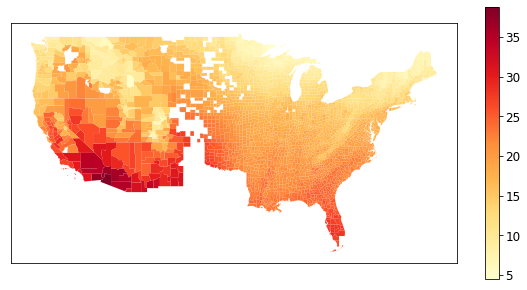
\includegraphics[width=.8\linewidth]{"./fig_lst.png"}
  \caption{\label{fig:lst} NASA MODIS Land Surface Temperature: Mean across county and most recent USDA FS panel ($^\circ$C)}
\end{figure}

\begin{figure}[!htbp]
  \centering
  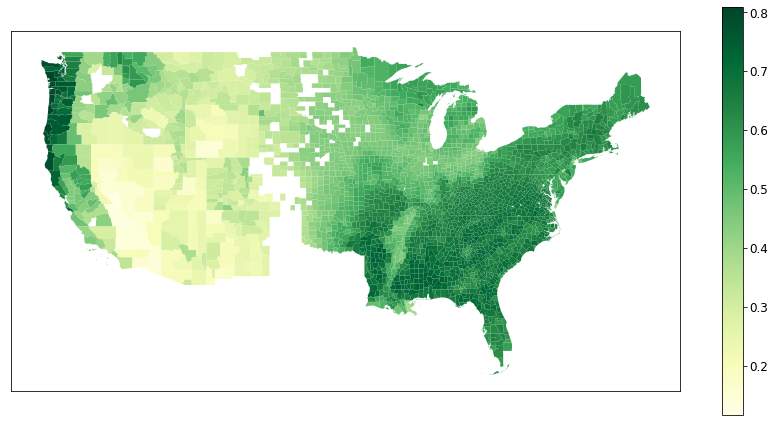
\includegraphics[width=.8\linewidth]{"./fig_ndvi.png"}
  \caption{\label{fig:ndvi} NASA MODIS NDVI: Mean across county and most recent USDA FS panel (unitless)}
\end{figure}

\begin{figure}[!htbp]
  \centering
  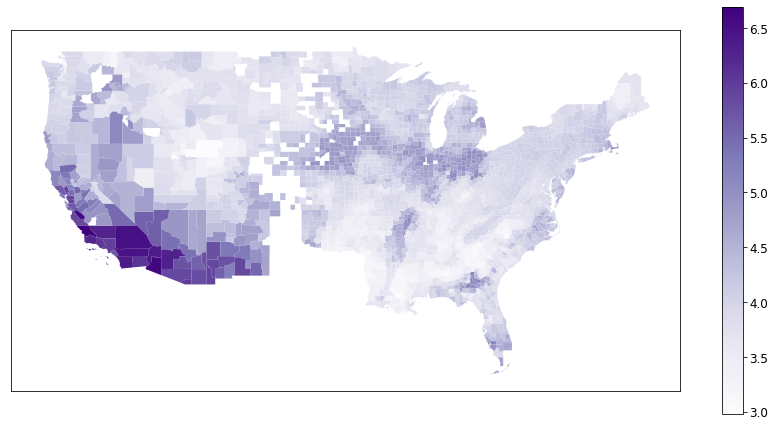
\includegraphics[width=.8\linewidth]{"./fig_cmbm.png"}
  \caption{\label{fig:cmbm} NASA MODIS NDVI: Consecutive months below average NDVI per year across county and most recent USDA FS panel'}
\end{figure}

%------------------------------------------------------------------------
\section{Methods}
\label{sec:methods}

I begin this research with regression analysis to understand the relationship between my remote sensing feature variables and the forest biomass measurement target variable. I then use several cross validation approaches to evaluate the performance of a statistical model under several distinct use cases.

\subsection{Regression analysis}
I use LASSO regularization paths to first visualize, then identify the importance of features in my feature space. LASSO regularization paths plot the magnitude of coefficients in a LASSO regression with varying values of the regularization tuning parameter \cite{hastietibs}. 

I then select the six most influential variables from this analysis and use these to run a simple OLS regression. My aim with this exercise is to pare down my feature space while maintaining the performance of my model, to help me interpret the coefficients of my regression.

\subsection{Model optimization}
I aim to develop models to predict forest biomass for three distinct use cases: predicting in regions with existing measurements, predicting in regions without existing measurements, and predicting forward in time. I describe how I optimize models for each of these distinct tasks below.

First, to optimize a model for predicting forest biomass in regions with existing measurements, I develop a K-fold county cross validation approach. I begin by holding out 10\% of counties for final model evaluation. With the remaining data, I implement a grouped five-fold cross validation strategy. This grouped k-fold ensures that all panels for each county only appear in a single fold, thus ensuring that each county-panel prediction is made with a model that has not yet seen any data from that county. Next, to optimize a model for predicting forest biomass in regions without existing measurements, I develop a state leave-one-out approach. I begin by holding out 5 states at random (chosen with weight proportional to number of counties in the state) for final model evaluation. With the remaining data, I hold out a single state at a time, train the model on the remaining states, and predict forest biomass in each county within the held-out state. Finally, to optimize a model for predicting forest biomass in future time panels, I first hold out the last panel from each county for final model evaluation. With the remaining data, I perform cross validation where I leave out one of the panels of data in each fold. For reference, each state has between one and four panels of data, so this results in 3 distinct folds. 

In each of these splitting strategies, I consider the best model to be the one with lowest prediction error as determined by root mean squared error (RMSE). This metric best aligns with the ultimate objective of this model, which is to make the best county-level predictions of forest biomass from remote sensing data. For robustness, I also evaluate mean absolute error (MAE) and the coefficient of determination ($R^2$) across all models.

In all splitting regimes, I begin by training two baseline models, which I expect to perform least well. These are intended to serve as a standard against which I can aim to improve predication error through the use of machine learning models. The first baseline model I consider is the simple global mean at each county-panel. The second baseline model I consider a simple linear regression of all predictor variables on county-level forest biomass predictions. I next optimize 4 machine learning models: Regularized linear regression (with Elastic Net), Simple Decision Trees, Random Forests, and XGBoost. I optimize the hyperparameters associated with each of these models through a grid search approach.

%------------------------------------------------------------------------
\section{Results}
\label{sec:results}

\subsection{Regression analysis}
The results of my LASSO path parameter selection exercise are presented in Figure \ref{fig:lasso}. Here I observe several key variables emerge with high coefficients under a high regularization constant (left-most side of the graph), and their coefficients continue to increase as the regularization constant decreases (moving right along the graph). The six variables that emerge strongest are the LST consecutive months below the mean, NDVI mean annual standard deviation, LST mean annual standard deviation, LST mean annual minimum, NDVI standard deviation of the annual mean, and NDVI standard deviation of the annual maximum. 

\begin{figure}[!htbp]
  \centering
  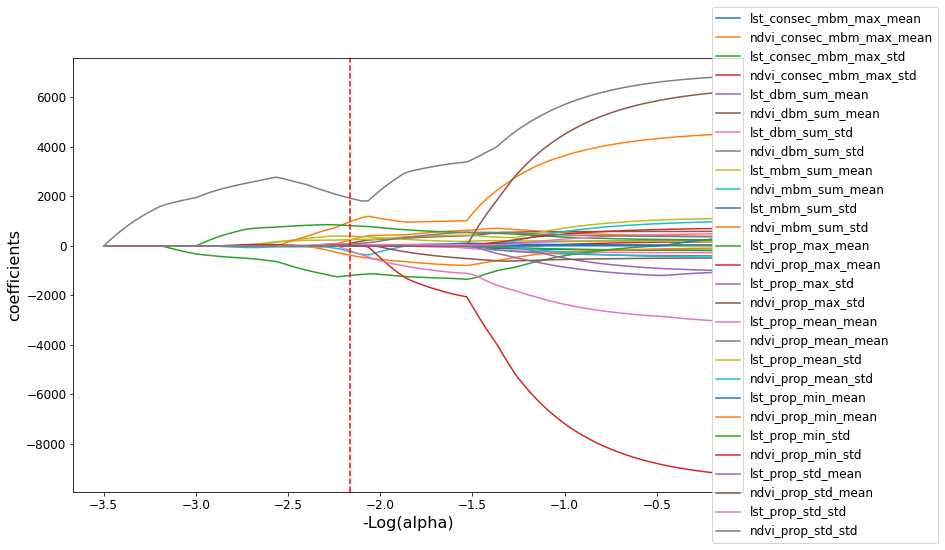
\includegraphics[width=.8\linewidth]{"./fig_lasso.png"}
  \caption{\label{fig:lasso} Lasso path parameter selection}
\end{figure}

I run an OLS regression of these six features on forest biomass and achieve a coefficient of determination of 0.60. The coefficient of determination reveals the portion of all variability in forest biomass that can be explained by these six features. From the coefficients in this model, I observe that more variable LST and NDVI is associated with lower forest biomass, and that a higher minimum LST is associated with lower forest biomass. The results of this regression are presented in Table \ref{tab:ols}.

\begin{table}[!htbp]
  \small
  \begin{center}
    \begin{tabular}{lrrrrrr}
    & \textbf{coef} & \textbf{std err} & \textbf{t} & \textbf{P$> |$t$|$} & \textbf{[0.025} & \textbf{0.975]}  \\
    \midrule
    \textbf{lst\_consec\_mbm\_max\_mean} &     671.5220  &       36.327     &    18.485  &         0.000        &      600.312    &      742.732     \\
    \textbf{ndvi\_prop\_std\_mean}       &   -2259.3378  &       64.492     &   -35.033  &         0.000        &    -2385.758    &    -2132.918     \\
    \textbf{lst\_prop\_std\_mean}        &   -6944.6139  &       71.098     &   -97.676  &         0.000        &    -7083.984    &    -6805.243     \\
    \textbf{lst\_prop\_min\_mean}        &   -7254.5791  &       94.628     &   -76.665  &         0.000        &    -7440.073    &    -7069.086     \\
    \textbf{ndvi\_prop\_mean\_std}       &     -63.0240  &       57.372     &    -1.099  &         0.272        &     -175.487    &       49.439     \\
    \textbf{ndvi\_prop\_max\_std}        &    -294.3720  &       57.017     &    -5.163  &         0.000        &     -406.140    &     -182.604     \\
    \textbf{const}                       &    4916.7393  &       30.013     &   163.820  &         0.000        &     4857.906    &     4975.572     \\
    \bottomrule
    \end{tabular}
    \end{center}
    \caption{\label{tab:ols} OLS regression with top 6 features emerging from lasso path analysis}
\end{table}

\subsection{Model selection}
I use cross validation to select the best set of hyper parameters for each model in each splitting regime. I find that the Random Forest Regressor yields the lowest RMSE (or is at parity with the lowest RMSE) in cross validation across all three splitting regimes. I present my model selection analysis in Table \ref{tab:modelselection}

\begin{table}[!htbp]
  \small
  \begin{center}
    \begin{tabular}{llrrr}
      \toprule
      Split regime &                                             Model &     RMSE &      MAE &   $R^2$ \\
      \midrule
      countyKFold &                                   DummyRegressor &  4399.24 &  3554.85 &  -0.00 \\
      countyKFold &                                 LinearRegression &  2002.37 &  1470.87 &   0.79 \\
      countyKFold &                                       ElasticNet &  2183.51 &  1612.81 &   0.75 \\
      countyKFold &                            DecisionTreeRegressor &  1750.86 &  1164.95 &   0.84 \\
      \textbf{countyKFold} &                            \textbf{RandomForestRegressor} &  \textbf{1425.77} &   \textbf{937.23} &   \textbf{0.89} \\
      countyKFold &                                     XGBRegressor &  1478.04 &   983.17 &   0.89 \\
      \midrule
      stateLOO &                                   DummyRegressor &  4630.31 &  4040.33 & -29.38 \\
      stateLOO &                                 LinearRegression &  2255.10 &  1768.55 &  -2.37 \\
      stateLOO &                                       ElasticNet &  2444.80 &  1933.84 &  -6.70 \\
      stateLOO &                            DecisionTreeRegressor &  1999.75 &  1485.87 &  -0.93 \\
      \textbf{stateLOO} &                            \textbf{RandomForestRegressor} &  \textbf{1621.44} &   \textbf{1227.17} &   \textbf{-0.74} \\
      stateLOO &                                     XGBRegressor &  1691.55 &  1284.28 &  -0.71 \\
      \midrule
      lastReport &                                   DummyRegressor &  3880.42 &  3234.15 &  -0.19 \\
      lastReport &                                 LinearRegression &  1874.07 &  1397.22 &   0.73 \\
      lastReport &                                       ElasticNet &  2006.74 &  1513.82 &   0.69 \\
      lastReport &                            DecisionTreeRegressor &  1773.12 &  1113.92 &   0.77 \\
      \textbf{lastReport} &                            \textbf{RandomForestRegressor} &  \textbf{1474.71} &   \textbf{900.80} &   \textbf{0.84} \\
      lastReport &                                     XGBRegressor &  1466.28 &   925.23 &   0.84 \\
      \bottomrule
      \end{tabular}
    \end{center}
    \caption{\label{tab:modelselection} Model selection: results from cross validation}
  \end{table}

\subsection{Model evaluation}
With the selected models presented above, I use my held-out test data to evaluate each. I first evaluate prediction accuracy using RMSE, MAE, and the coefficient of determination. I then examine the linear relationship between predictions and true values. And lastly, I perform several statistical tests for two-sample comparisons with the goal of assessing the likelihood that predictions and the test data came from the same datset. 

My data splitting scenarios resulted in a test dataset of 10\% at random for county k-fold regime, a test dataset of 12.9\% (including all of AL, MN, OH, and WI) for my state leave-one-out regime, and a test dataset of 32\% for my future prediction regime.

In all three of my splitting regimes, I find that my selected models perform well. In each case, RMSE is not significantly higher than it was in my cross validaiton exercise, giving me confidence that these models are likely not overfit. RMSE on the test dataset was 1136, 1547, and 1596 short tons / km2 respectively; $R^2$ was 0.92, 0.74, and 0.89 respectively; and MAE was 822, 1109, and 1068 short tons / km2 respectively. I present the comparisons between true and predicted values across these three regimes in Figure \ref{fig:testreg}.

\begin{figure}[!htbp]
  \centering
  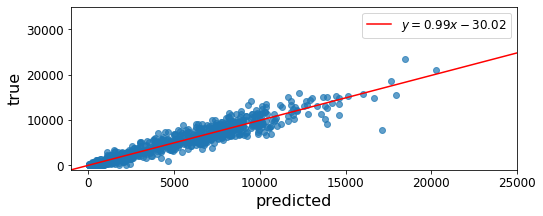
\includegraphics[width=.8\linewidth]{"./fig_regcounty.png"}
  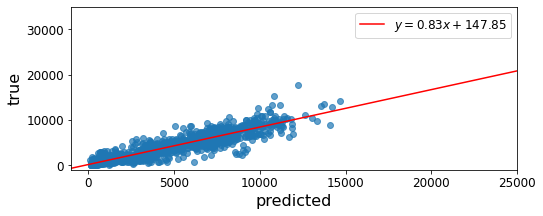
\includegraphics[width=.8\linewidth]{"./fig_regstate.png"}
  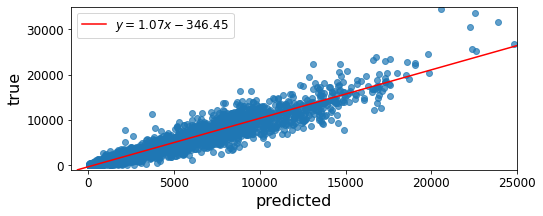
\includegraphics[width=.8\linewidth]{"./fig_regfuture.png"}
  \caption{\label{fig:testreg} Performance on test data for (top to bottom) county K-fold, state LOO, future prediction}
\end{figure}

\begin{table}[!htbp]
  \small
  \begin{center}
    \begin{tabular}{llll}
    \textbf{Test (p-value)} & \textbf{County k-fold} & \textbf{State LOO} & \textbf{Future pred}\\
    \bottomrule
    Levene equal variance & 0.5158 & 0.0000** & 0.0000**\\
    Paired t-test & 0.5489 & 0.0000** & 0.0000**\\
    Signed rank test & 0.1945 & 0.0000** & 0.0423\\
    \bottomrule
    \end{tabular}
    \end{center}
    \caption{\label{tab:twosample} Two sample comparison tests ($H_0$: not different)}
\end{table}

To conclude this analysis, I perform a Levene equal variance test, paired t-test, and signed rank test between each prediction dataset and the held-out test data to evaluate the likelihood of the prediciton data coming from the same distribution as the test data, summarized in Table \ref{tab:twosample}. These metrics can help justify the use of my selected models for predictions over a broader scale than simply a county. I find that I cannot reject the null hypothesis that the samples come from the same distribution in the county k-fold regime, however the tests for differences are significant in both the state leave-one-out and future prediction regimes. This makes me less confident about using these latter two models for making population-level predictions out of region or into the future. I include histograms of predictions and my test data in Figure \ref{fig:testhist}.

\begin{figure}[!htbp]
  \centering
  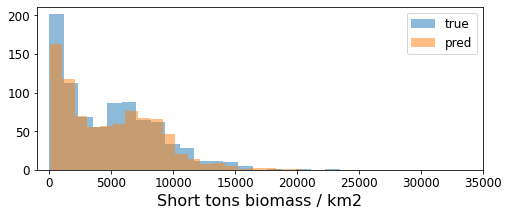
\includegraphics[width=.8\linewidth]{"./fig_histcounty.png"}
  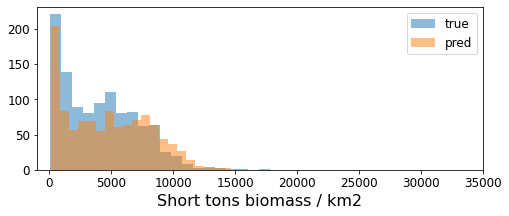
\includegraphics[width=.8\linewidth]{"./fig_histstate.png"}
  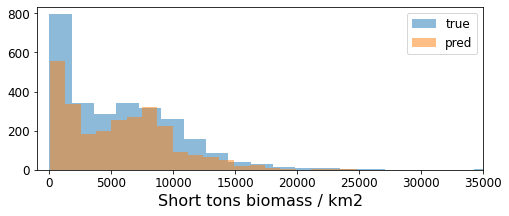
\includegraphics[width=.8\linewidth]{"./fig_histfuture.png"}
  \caption{\label{fig:testhist} Histogram of forest biomass predictions for (top to bottom) county K-fold, state LOO, future prediction}
\end{figure}

%------------------------------------------------------------------------
\section{Conclusion}
In this research I explore the viability of statistical models to quantify forest biomass. These models leverage a current datasets of forest biomass measurement, collected through intensive sampling campaigns run by the USDA Forest Service, to produce higher frequency estimates with the help of low-cost remote sensing data. 

I find that several aggregated remote sensing features can be predictive of county-panel-level forest biomass, achieving an $R^2$ of 0.60. Specifically, more variable land surface temperature and NDVI are associated with lower forest biomass, and a higher minimum land surface temperature is associated with lower forest biomass.

My aim with these statitical models is to support predictions under three scenarios: in regions with existing measurements, in regions without existing measurements, and forward in time. I find that the Random Forest Regressor yields the lowest RMSE in cross validation across all three splitting regimes. In all three of my splitting regimes, I find that my selected models perform well in predicting on held-out data (RMSEs of 1136, 1547, and 1596 short tons / km2 respectively). In each case, RMSE is not significantly higher than it was in my cross validaiton exercise, giving me confidence that these models are likely not overfit. 

Lastly, I find that I cannot reject the null hypothesis that the samples come from the same distribution in the county k-fold regime, however the tests for differences are significant in both the state leave-one-out and future prediction regimes. This makes me less confident about using these models for making population-level predictions out of region or into the future.

%------------------------------------------------------------------------
\section*{Broader impact}

This research contributes to the larger field of forest biomass quantification. On the whole, improved approaches to forest monitoring will support humans' care for this natural resource. 

While a central component of this paper focuses on estimate uncertainty, it is often the case for downstream users to use estimates without consideration of their uncertainty. When these forest biomass estimates are used in carbon markes or other in governmental or corporate statements without uncertainty qualifications, this can lead and has led to inflated claims of climate impact (a.k.a., "greenwashing").

Additionally, this research and the models in this paper directly benefit those countries and regions with better surveyed data. While remote sensing layers tend to have complete coverage of the Earth, the surveyed forest biomass as well as other potential predictors like soil types and crop layers tend to only be availble in wealthier countries. This translates to wealthier nations having access to more precise models and downstream economic and enviornmental benefits. That said, the contiguous United States has a variety of climactic regions and may be representative of large parts of the world, meaning these models might be able to translate to developing country scenarios. 

Beyond what is mentioned above, leveraging biases in the data is not applicable to this research. 

%------------------------------------------------------------------------
% REFERENCES
{\small
\bibliographystyle{ieee}
\bibliography{egbib}
}

\end{document}